
\subsection{Analysis of beam-on data}


\begin{table}[htbp]
\centering
\resizebox{\textwidth}{!}{%
\begin{tabular}{lccc}
\hline
Cut & Beam-off Events/h & Beam-on Events/h & Beam On/Beam Off Ratio \\
\hline
Initial & $2064.42 \pm 6.80$ & $2810.74 \pm 13.04$ & $1.36$ \\
Neutrino PFParticle in slice & $1954.79 \pm 6.61$ & $2649.18 \pm 12.66$ & $1.36$ \\
Vertex fiducial volume & $1144.34 \pm 5.06$ & $1248.59 \pm 8.69$ & $1.09$ \\
N daughter particles & $568.02 \pm 3.57$ & $589.28 \pm 5.97$ & $1.04$ \\
Max $\cos(\theta_{\mathrm{beam}})$ & $54.47 \pm 1.10$ & $69.29 \pm 2.05$ & $1.27$ \\
Cut on $C_{0-10}$ & $22.09 \pm 0.70$ & $27.75 \pm 1.30$ & $1.26$ \\
Cut on $C_{40-50}$ & $15.91 \pm 0.60$ & $19.77 \pm 1.09$ & $1.24$ \\
Cut on $C_{140-150}$ & $8.62 \pm 0.44$ & $13.66 \pm 0.91$ & $1.58$ \\
ROI Z size & $5.37 \pm 0.35$ & $9.98 \pm 0.78$ & $1.86$ \\
ROI Z close to vertex & $2.08 \pm 0.22$ & $6.35 \pm 0.62$ & $3.05$ \\
Tail Length Density & $0.67 \pm 0.12$ & $3.63 \pm 0.47$ & $5.42$ \\
\hline
\end{tabular}
}
\caption{Beam-on and beam-off events per hour with the corresponding ratio for various selection cuts, considering all the available time with the spill on.}
\label{tab:onoff_ratio_alltps}
\end{table}

After defining the selection criteria as described in the previous section, the data collected with the beam on, where neutrino candidates are expected, 
was analyzed and compared to the runs with beam off, where only background is expected. The number of events per hour after each stage of the selection is shown 
in Table~\ref{tab:onoff_ratio_alltps}.
The event rate per hour in the beam-on data is significantly higher than that observed in the beam-off data, indicating the presence of neutrino interactions related to beam activity. 
% However, the measured rate remains lower than the expectation from the Monte Carlo simulation. 
% This discrepancy can be attributed to the limited statistical sample as well as to systematic uncertainties arising from the neutrino flux (hadron production), interaction cross sections, beamline instrumentation, and detector response. 
% A detailed evaluation of these effects is beyond the scope of the present analysis, which is focused on neutrino identification as a proof of principle for the BSM physics program.

The measured rate is compatible with the expectation of the Monte Carlo simulation, but it's important to keep in mind that there are sources of systematic uncertainties (neutrino flux, interaction cross sections, beamline instrumentation, and detector response) that would require a detailed evaluation, which is beyond the scope of the present analysis, which is focused on neutrino identification as a proof of principle for the BSM physics program.



\begin{figure}[h]
    \centering
    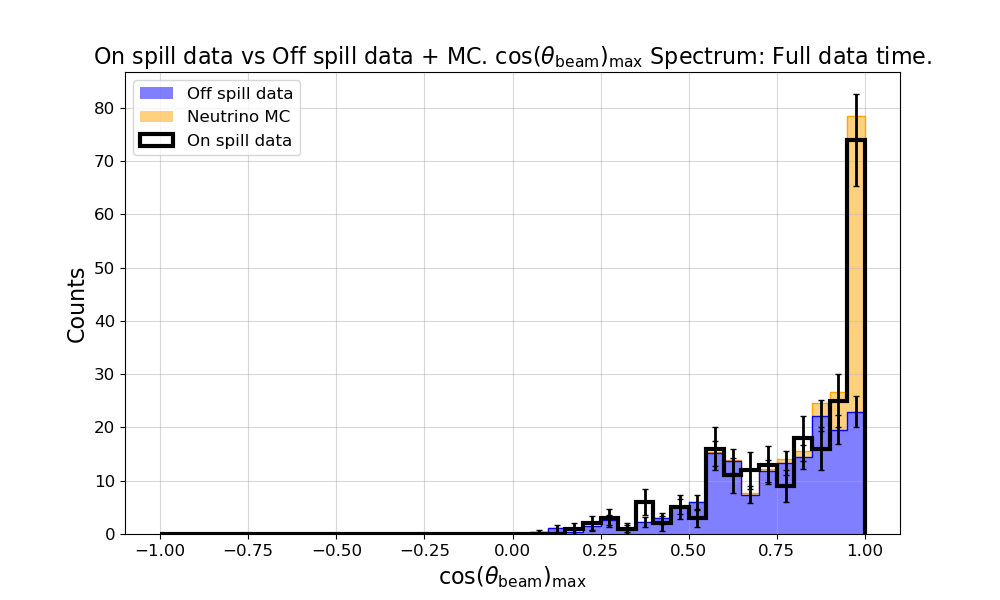
\includegraphics[width=0.69\linewidth]{sections/plots/version_2/beam_on_vs_off/output_test_full_time/sig_bkg_mc_max_directionZ_directionZ2_spectrum_full_sig_time.png}
    \caption{Distribution of $\cos(\theta_{\mathrm{beam}})_\text{max}$ comparing beam-on data with the stacked distributions of beam-off and Monte Carlo neutrinos.}
    \label{fig:beam_on_maxZ_all_tps}
\end{figure}

A key cross-check is the comparison of the $\cos(\theta_{\mathrm{beam}})_\text{max}$ distribution with and without beam (Figure~\ref{fig:beam_on_maxZ_all_tps}), where a clear excess in the forward direction is visible with the beam on.


\begin{figure}[h]
    \centering
    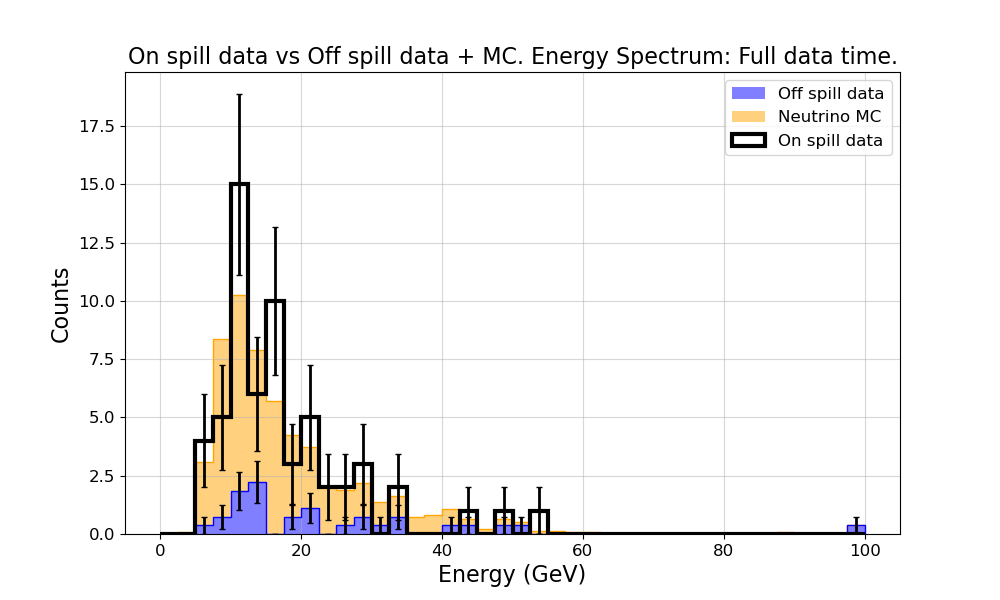
\includegraphics[width=0.69\linewidth]{sections/plots/version_2/beam_on_vs_off/output_test_full_time/sig_bkg_mc_energy_spectrum_full_sig_time.png}
    \caption{Deposited Energy spectrum comparing beam-on data with the stacked distributions of beam-off and Monte Carlo neutrinos.}
    \label{fig:beam_on_energy_all_tps}
\end{figure}

Additional distributions are used to check MC–data agreement, starting with the energy spectrum (Figure~\ref{fig:beam_on_energy_all_tps}), for which no cut is applied. %; the shapes appear compatible by eye, though the limited statistics preclude stronger statements. 
For a broader overview, multiple variables are compared (Figs.~\ref{fig:all_tps_beam_on_tail_density}, 
\ref{fig:all_tps_beam_on_energyDepositedInFifteenth10cm}, \ref{fig:all_tps_beam_on_distance_vertexZ_to_ROI_start},
\ref{fig:all_tps_beam_on_numberOfPFParticles}, \ref{fig:all_tps_beam_on_vertexY}, \ref{fig:all_tps_beam_on_vertexZ}, 
\ref{fig:all_tps_beam_on_energyDepositedInFifth10cm}, \ref{fig:all_tps_beam_on_ROI_Z_size}, \ref{fig:all_tps_beam_on_energyDepositedInFirst10cm})
, where it is possible to see hints of good agreement between the shape of the expected distributions and the data despite the low statistics available. 

    Given the ProtoDUNE Horizontal Drift active volume (3.6 m maximum drift, active detector dimensions of order a few meters), muons produced in the selected high-energy neutrino interactions (candidate energies typically above 10 GeV, GENIE kinetic energies up to 120 GeV in the simulated sample) are frequently not contained within the TPC and exit through the detector boundary before depositing their full energy. This is consistent with the reconstructed "Total direction" variable (Section 6.3), where the outgoing muon's momentum is often missing from the reconstructed final state.\\
    The consequence for this analysis is twofold. First, the calorimetric-hits energy reconstruction (Section 6.2) — which sums deposited charge within the reconstructed slice — systematically underestimates the true neutrino energy for events with an exiting muon, since only the contained fraction of the muon track contributes to the deposited-energy sum; this should be kept in mind when comparing the reconstructed energy spectrum (Figure 25) to GENIE-level expectations. Second, because the selection cuts (C0-10, C40-50, C140-150) are defined from charge deposited in fixed-distance bins near the reconstructed vertex rather than from the full track, muon non-containment does not directly bias the vertex-region selection, but it does mean the deposited-energy variable used for cross-checks is a lower bound rather than a full energy measurement. A dedicated muon-track/containment-based selection is identified as a direction for future work.


After all the selections, the final number of events is 60 ($\text{N}_{\text{ON}}$)  within the 16.5387 hours ($\text{T}_{\text{ON}}$) of beam on and 30 ($\text{N}_{\text{OFF}}$) in the 44.6886 hours ($\text{T}_{\text{OFF}}$) of beam off, as reported in Table~\ref{tab:post_cut_numbers_all_tps}.

\begin{figure}[h]
    \centering
    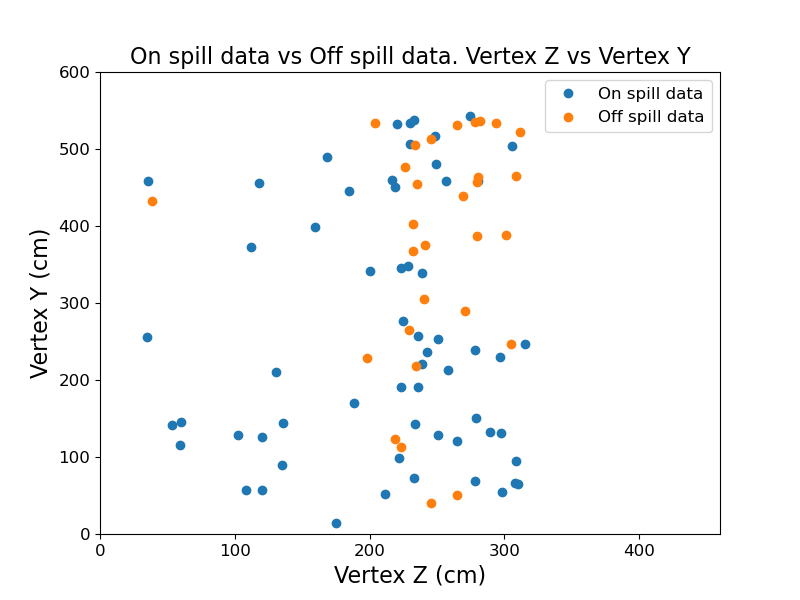
\includegraphics[width=0.69\linewidth]{sections/plots/version_2/beam_on_vs_off/sig_bkg_vertexZ_vs_vertexY_scatter.png}
    \caption{Vertex position in the ZY plane for the spill-on and spill-off events that pass all selections, considering all the available spill on time.}
    \label{fig:vertex_position_yz_all_tps}
\end{figure}

It is interesting to observe the position of the vertices in the detector for the events that pass all the selections (Figure \ref{fig:vertex_position_yz_all_tps}), where we see a certain preference in the lower part of the detector for the events with the beam on, while the cosmic events collected with the spill off tend to occur more in the upper section, as expected from the MC simulations.  
One can also see a higher efficiency in the downstream region of the detector, justified by the APA 1 collection plane not working perfectly. 
Standard Model particles different from neutrinos are expected to interact more in the upstream section of the detector, so the absence of this behavior is a hint confirming these events are neutrinos.



\clearpage



\subsection{Significance calculation} \label{chap:significance_method}

\begin{table}[htbp]
    \centering
    \begin{tabular}{|c|c|c|c|}
        \hline
         & Number of events & Time (hours) & Hourly rate\\
        \hline
        Beam-on & 60 & 16.5387 & 3.63 \\
        \hline
        Beam-off & 30 & 44.6886 & 0.67\\
        \hline
    \end{tabular}
    \caption{Observed number of events that pass all selection cuts, and total live time available.}
    \label{tab:post_cut_numbers_all_tps}
\end{table}


An excess of events with the beam on is clearly visible by eye, but a precise calculation of its significance is needed.

At first, the significance of the excess is simply computed using the basic significance formula for Poissonian-distributed events
\begin{equation} \label{eq:basic_formula}
    \chi^2 = 2 \left(  \mu- \text{Data}_{\text{ON}} + \text{Data}_{\text{ON}} \ln \frac{\text{Data}_{\text{ON}}}{\mu}\right) \, ,
\end{equation}
where $\mu = \text{Data}_{\text{OFF}} \cdot \frac{\text{Time}_{\text{ON}}}{\text{Time}_{\text{OFF}}}$. 
Using the number of events shown in Table~\ref{tab:post_cut_numbers_all_tps} we obtain a significance of $10.23\sigma$.

The simple approach only considers the case where the background rate is exactly the measured value $\frac{\text{Data}_{\text{OFF}}}{\text{Time}_{\text{OFF}}}$, but it can be interesting to use a different approach to explore the entire space of the signal and the background rates and to find the credible intervals for the experiment. 

The idea is to find the optimal values for the neutrino and background rates by sampling the likelihood distribution, where the likelihood is defined as:
\begin{equation}\label{eq:likelihood}
    \mathcal{L}_{\text{Poisson}}
    = \mathcal{L}_{\text{Poisson, ON}} \times \mathcal{L}_{\text{Poisson, OFF}}
    = \frac{e^{-\text{Model}_{\text{ON}}}\,\text{Model}_{\text{ON}}^{\text{Data}_{\text{ON}}}}{\text{Data}_{\text{ON}}!}
      \times
      \frac{e^{-\text{Model}_{\text{OFF}}}\,\text{Model}_{\text{OFF}}^{\text{Data}_{\text{OFF}}}}{\text{Data}_{\text{OFF}}!}\,,
\end{equation}
where \(\text{Model}_{\text{ON}}=(\text{R}_{\text{neutrino}}+\text{R}_{\text{background}})\cdot \text{Time}_{\text{ON}}\) and \(\text{Model}_{\text{OFF}}=\text{R}_{\text{background}}\cdot \text{Time}_{\text{OFF}}\), and $\text{R}$ is defined as the event rate per hour.


\begin{figure}[h]
    \centering
    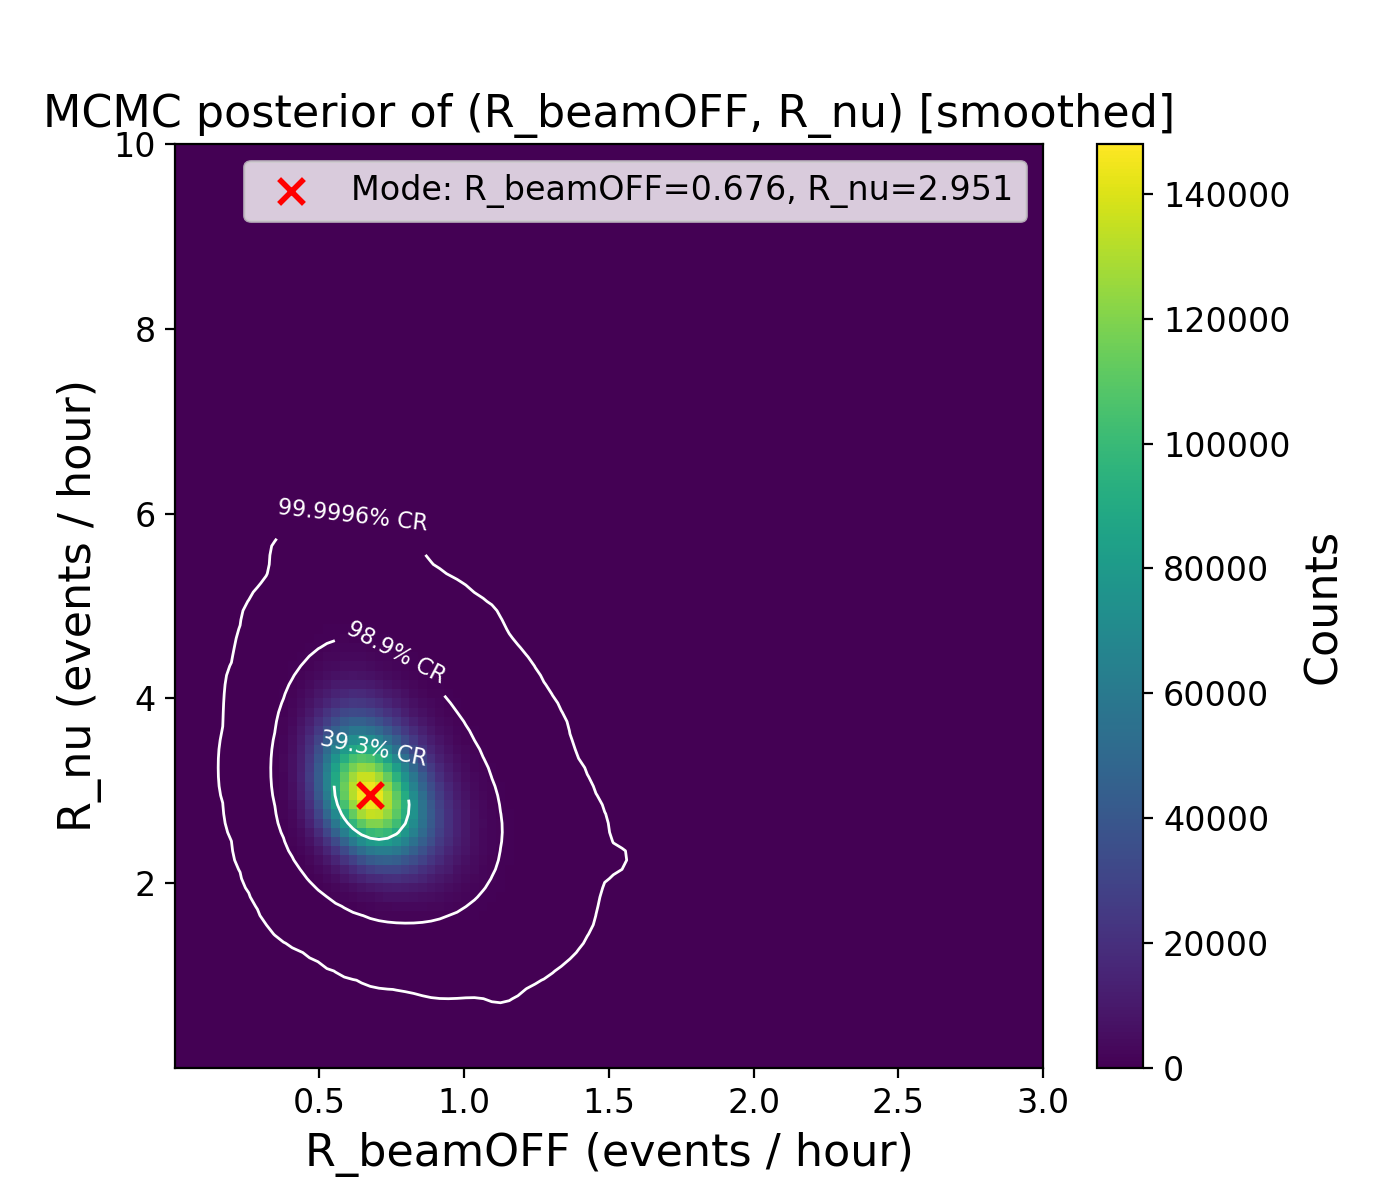
\includegraphics[width=0.69\linewidth]{sections/results/plots/significance/mcmc_posterior_contours_smoothed.png}
    \caption{Histogram of the sampled \(\log(\mathcal{L}_{\text{Poisson}})\) using the Monte Carlo method. Contours are drawn using the 0.393, 0.989, and 0.999996 quantiles.}
    \label{fig:mcmc_approach_all}
\end{figure}
 
The chosen approach samples the log-likelihood distribution (Eq.~\ref{eq:likelihood}) using a Markov Chain Monte Carlo (MCMC) method, using 100 walkers for $2\times10^5$ steps, discarding the first $2\times10^4$ steps as burn-in.
The contours are then drawn using the 0.393, 0.989, and 0.999996 quantiles (Figure~\ref{fig:mcmc_approach_all}). Assuming  flat priors these correspond, in a purely Bayesian way, to the credible regions at 39.3\%, 98.9\%, and 99.9996\% probability. % without the need of introducing any Gaussian approximation.
The most probable values are \(\text{R}_{\text{neutrino}}=2.951\) and \(\text{R}_{\text{background}}=0.676\), and the hypothesis \(\text{R}_{\text{neutrino}}=0\) falls outside of the credible region at 99.9996\% probability, for every plausible true \(\text{R}_{\text{background}}\).
\subsubsection{Impact of systematic Uncertainties}
The following fractional systematic uncertainties are considered:
\begin{itemize}
    \item Neutrino flux: $\sigma_{\rm flux} = 20\%$
    \item Neutrino cross-section: $\sigma_{\rm xsec} = 20\%$
    \item Detection efficiency: $\sigma_{\rm eff} = 10\%$
    \item Angular resolution: $\sigma_{\rm \theta} = 10\%$
    \item Detector effects: $\sigma_{\rm det} = 10\%$
    \item Background modeling: $\sigma_{\rm bkg} = 10\%$
\end{itemize}

The total combined uncertainties are evaluated in quadrature:
\begin{align}
    \sigma_{\rm signal} &= \sqrt{\sigma_{\rm flux}^2 + \sigma_{\rm xsec}^2 + \sigma_{\rm eff}^2 + \sigma_\theta^2 + \sigma_{\rm det}^2},\\
    \sigma_{\rm bkg} &= \sqrt{\sigma_{\rm bkg}^2 + \sigma_{\rm det}^2}.
\end{align}

The resulting 2D likelihood contours are shown in Figure~\ref{fig:likelihood_contours}. The black contours correspond to the no-systematics case, while the red dashed contours include quadrature systematic uncertainties. This systematics-inclusive recomputation is still pending for the new reconstruction; the figure below reflects the earlier, old-reconstruction result.

\begin{figure}[h!]
\centering
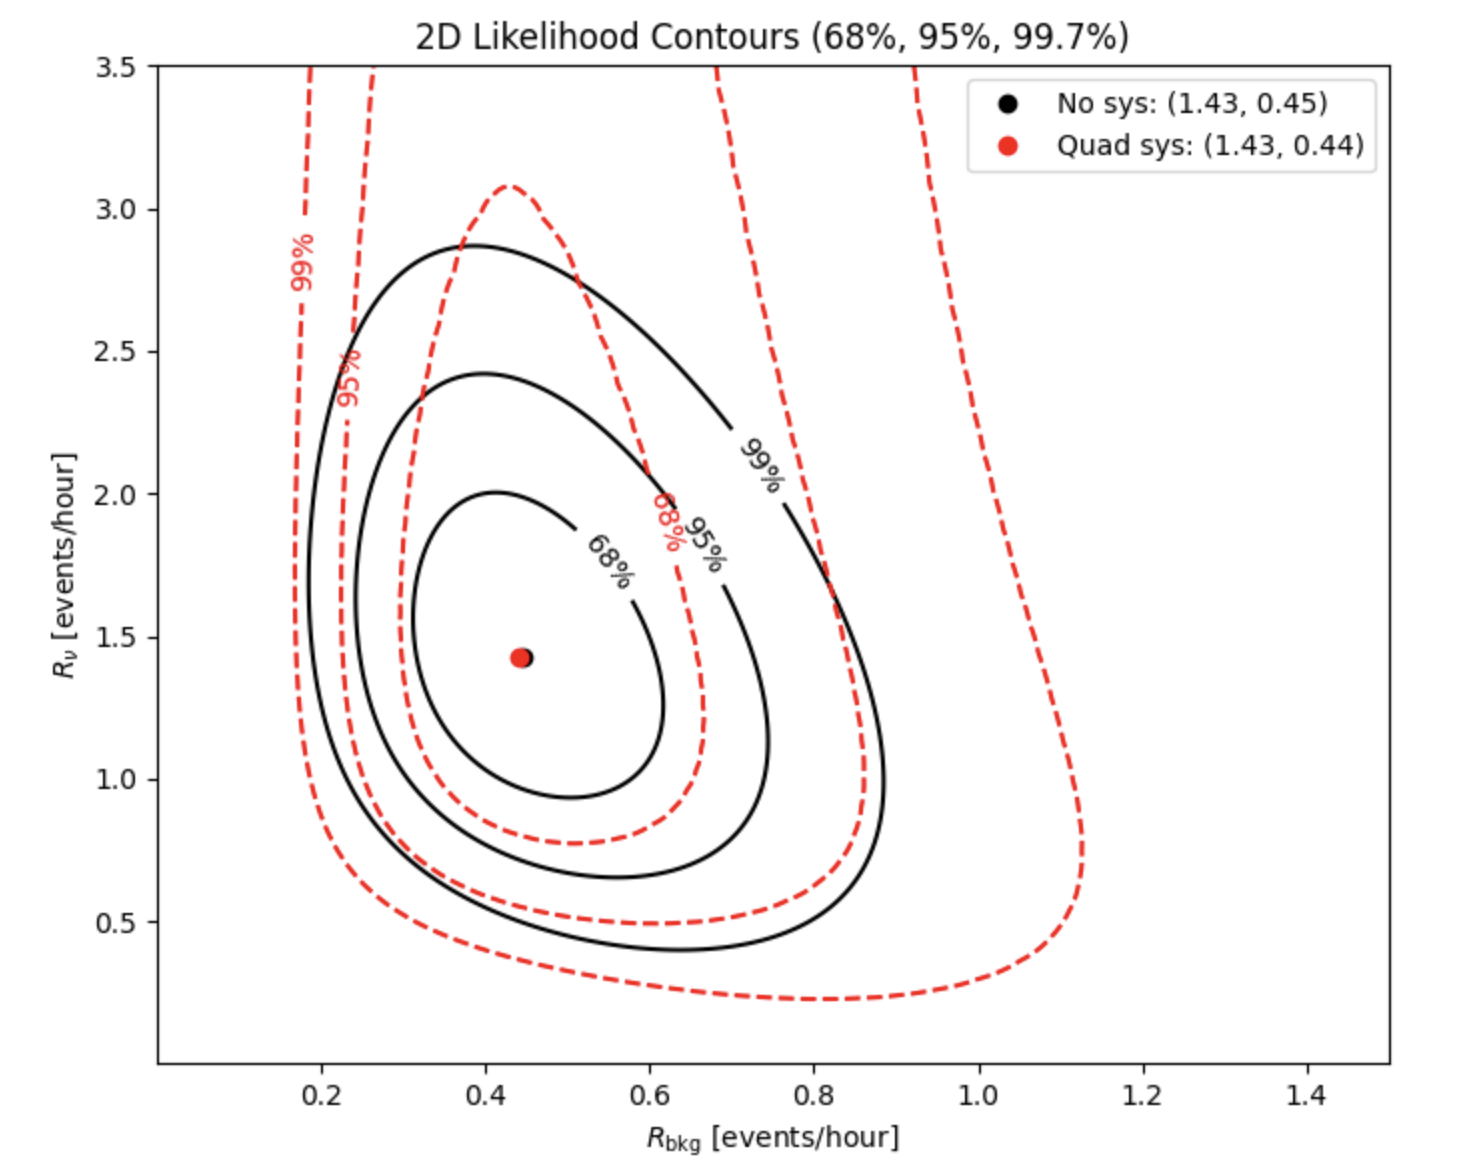
\includegraphics[width=0.7\textwidth]{sections/results/plots/significance/2D_Contours_WSys.png}
\caption{Two-dimensional likelihood contours for $R_\nu$ and $R_{\rm bkg}$. Levels correspond to 68\%, 95\%, and 99.7\% confidence regions. Black: no systematics; red dashed: quadrature systematics. The markers indicate the maximum likelihood estimates. Based on the old reconstruction; pending regeneration.}
\label{fig:likelihood_contours}
\end{figure}

The comparison between the no-systematics and quadrature-systematics contours shows that including reasonable systematic uncertainties slightly broadens the contours. However, the difference is small, indicating that the measurement is dominated by statistical uncertainty rather than systematics.

\subsection{Event displays}

These searches can really benefit from a visual confirmation with the event displays, to better understand the nature of the events that were selected with the analysis. Many events that pass the selection look like neutrino events, with clean vertices inside the detector and the correct direction parallel to the Z coordinate (Figure \ref{fig:ev_display}).
Among the events, cosmic events are also present, as expected. These events are easy to identify because they usually have shapes and topologies different from the expected neutrino ones (Figure \ref{fig:ev_display_err}). 
It is interesting to observe that certain events have a clear muon track preceding the shower. However, since the shower happens near the beginning of the APA2, the track in the APA1 is lost and the events are identified as neutrinos (Figure \ref{fig:ev_display_broken1}). 

\begin{figure}[h]
    \centering
    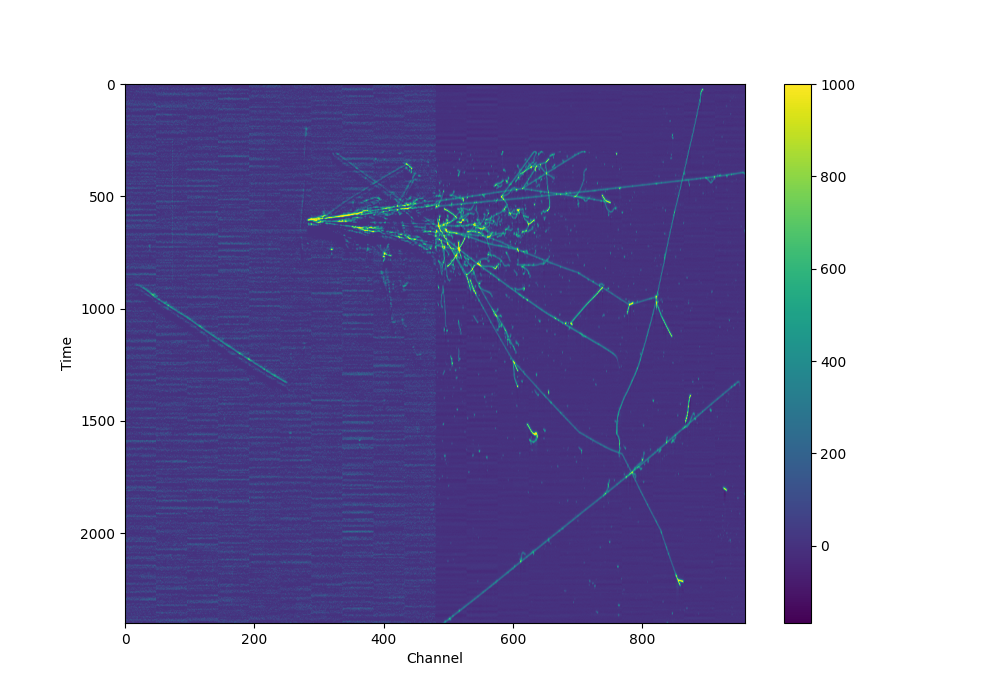
\includegraphics[width=0.48\linewidth]{sections/results/plots/ev_display/_full_collection_view_12_27099.png}
    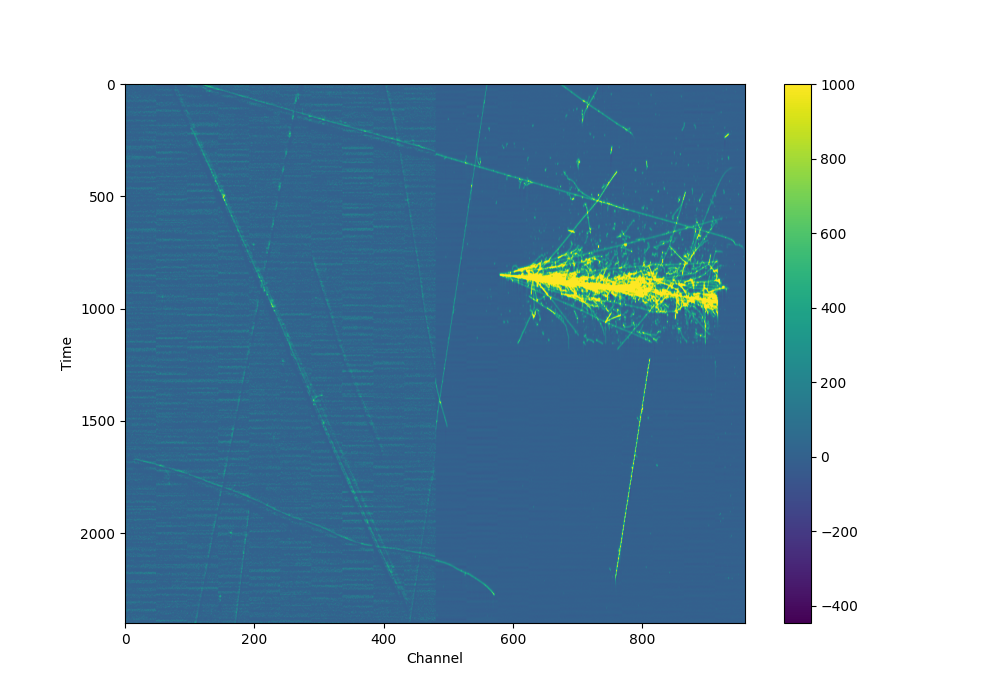
\includegraphics[width=0.48\linewidth]{sections/results/plots/ev_display/_full_collection_view_12_102658.png}
    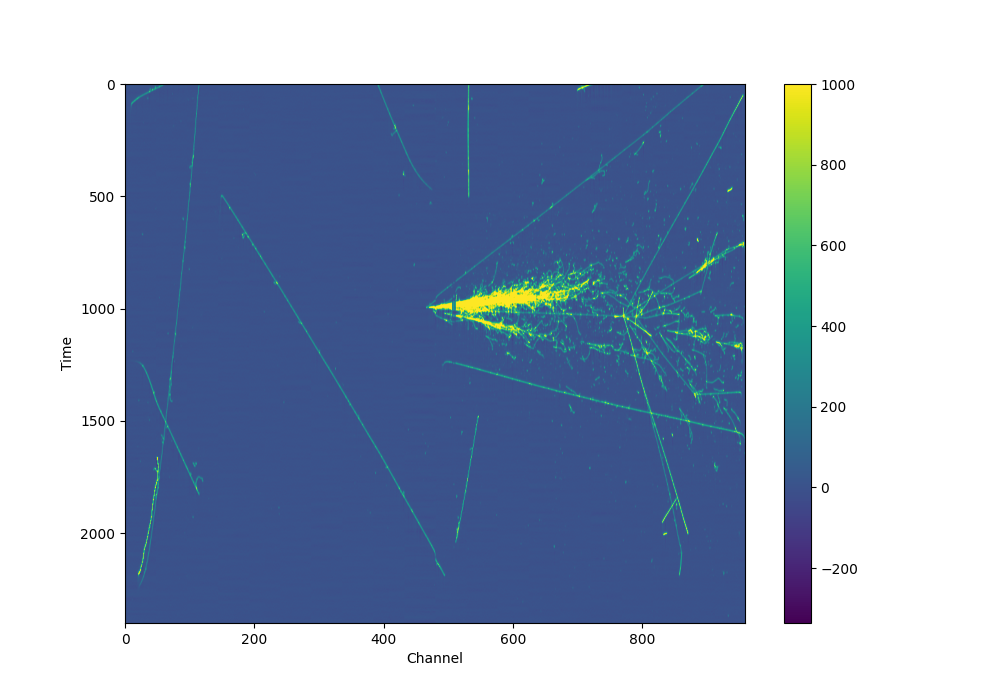
\includegraphics[width=0.48\linewidth]{sections/results/plots/ev_display/_full_collection_view_34_2914.png}
    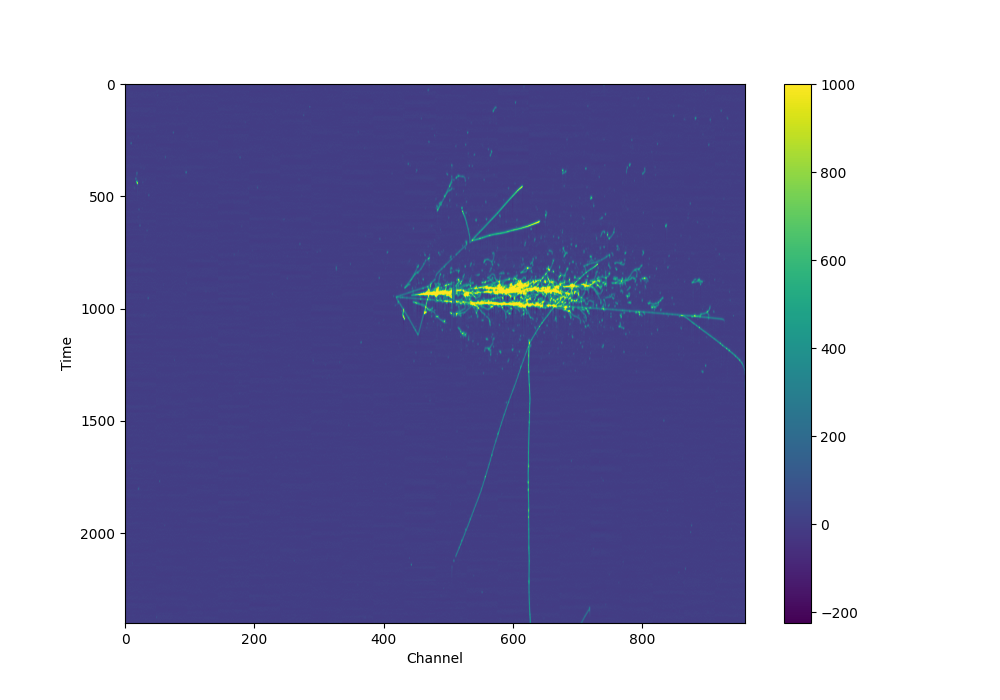
\includegraphics[width=0.48\linewidth]{sections/results/plots/ev_display/_full_collection_view_34_22541.png}
    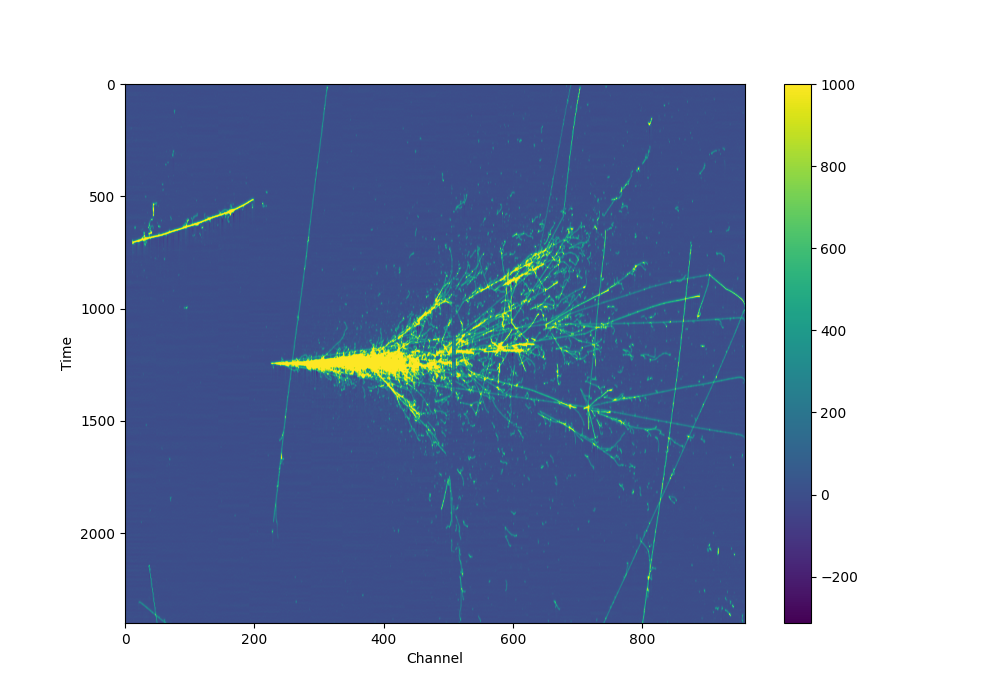
\includegraphics[width=0.48\linewidth]{sections/results/plots/ev_display/_full_collection_view_34_41861.png}
    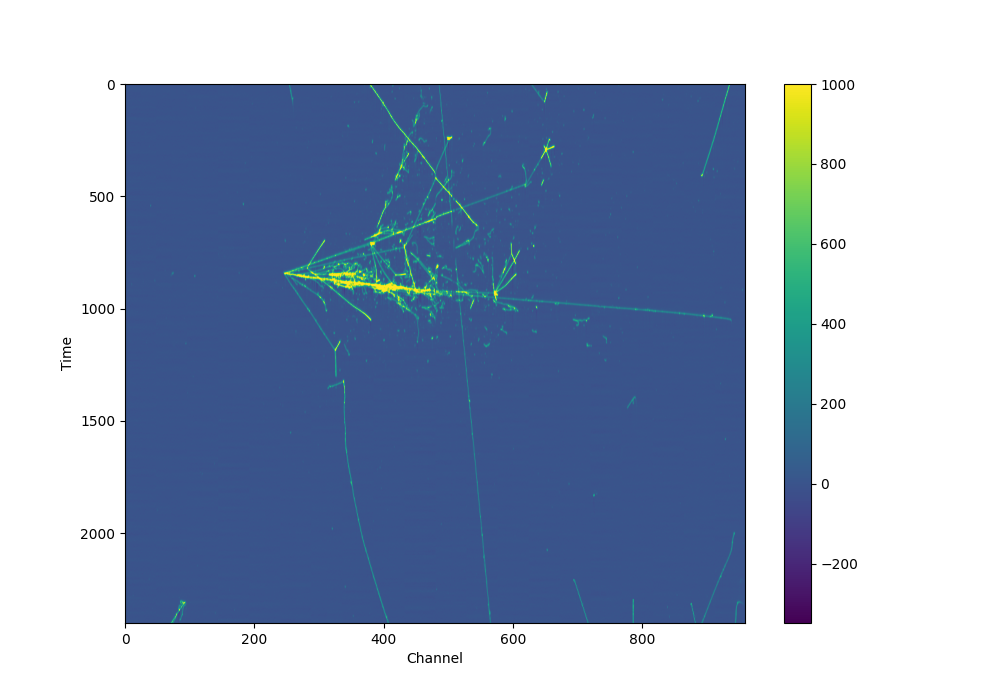
\includegraphics[width=0.48\linewidth]{sections/results/plots/ev_display/_full_collection_view_34_79161.png}
    \caption{Event displays of neighboring APAs’ collection view planes containing neutrino candidates.}
    \label{fig:ev_display}
\end{figure}

\begin{figure}[h]
    \centering
    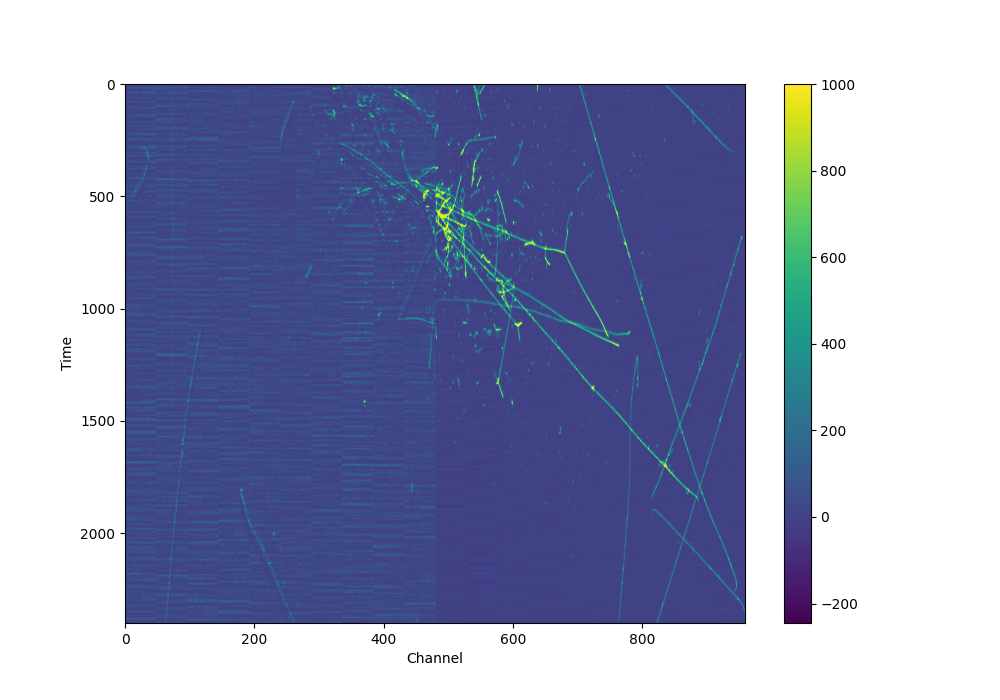
\includegraphics[width=0.48\linewidth]{sections/results/plots/ev_display/_full_collection_view_12_96338.png}
    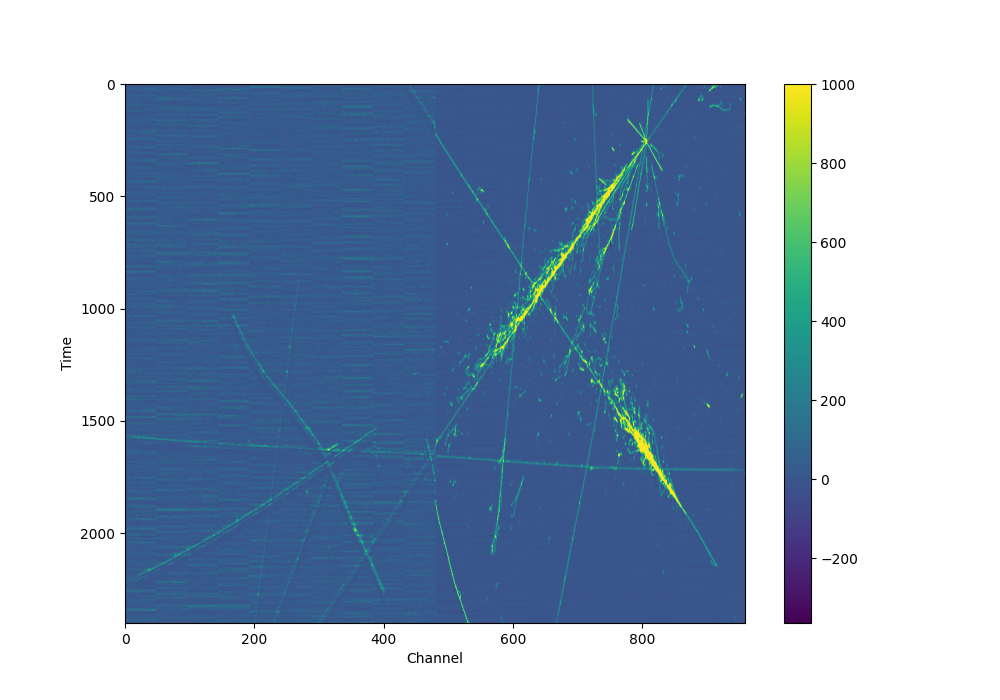
\includegraphics[width=0.48\linewidth]{sections/results/plots/ev_display/_full_collection_view_12_8703.png}
    \caption{Event displays of neighboring APAs’ collection view planes containing background events.}
    \label{fig:ev_display_err}
\end{figure}


\begin{figure}[h]
    \centering
    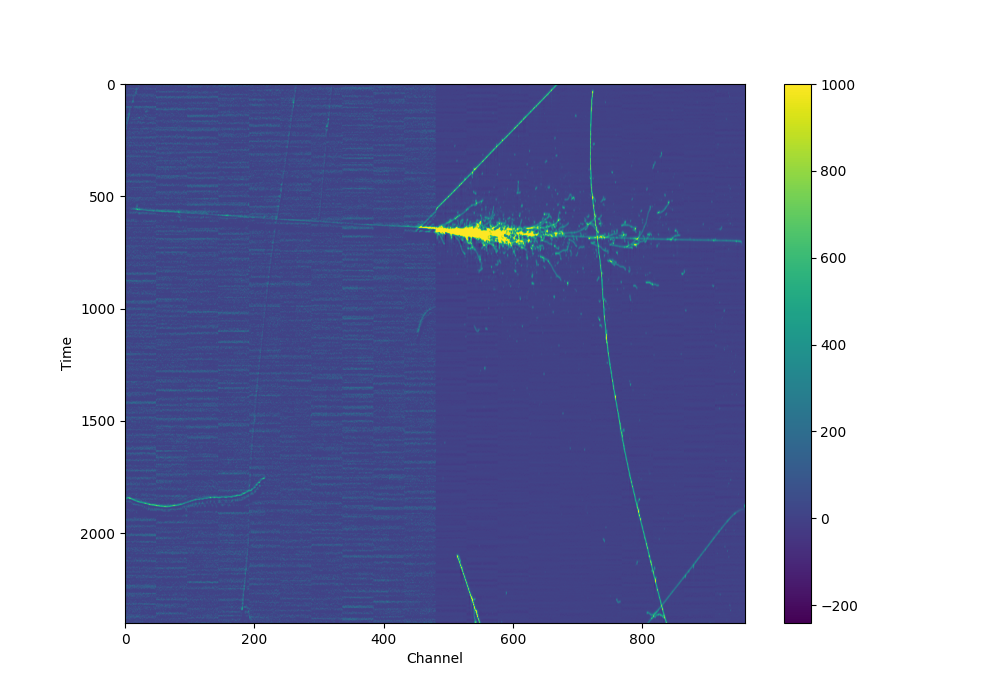
\includegraphics[width=0.48\linewidth]{sections/results/plots/ev_display/_full_collection_view_12_47601.png}
    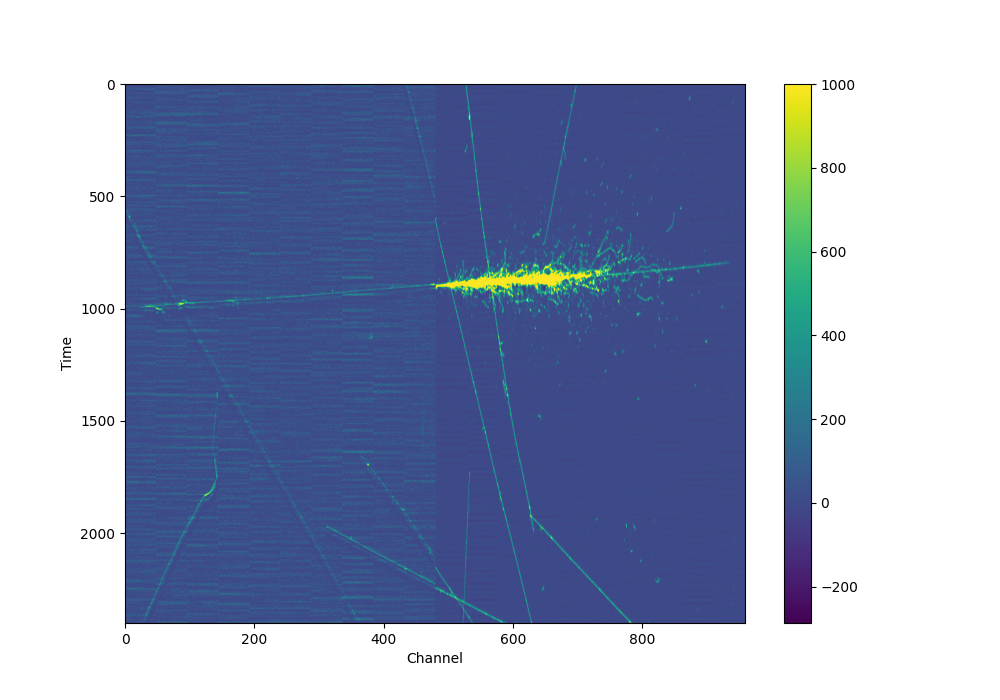
\includegraphics[width=0.48\linewidth]{sections/results/plots/ev_display/_full_collection_view_12_45228.png}
    \caption{Event displays of neighboring APAs’ collection view planes containing background events. The signal from the APA 1 is enhanced to make the activity more visible.}
    \label{fig:ev_display_broken1}
\end{figure}
\clearpage

\subsection{High TP vs Low TP validation}
\begin{table}[htbp]
\centering
\resizebox{\textwidth}{!}{%
\begin{tabular}{lccc}
\hline
Cut & Beam-off Events/h & Beam-on Events/h (High TP) & Beam-on Events/h (Low TP) \\
\hline
Initial & $2064.42 \pm 6.80$ & $3566.82 \pm 21.02$ & $2089.44 \pm 15.71$ \\
Neutrino PFParticle in slice & $1954.79 \pm 6.61$ & $3347.37 \pm 20.36$ & $1983.10 \pm 15.31$ \\
Vertex fiducial volume & $1144.34 \pm 5.06$ & $1340.11 \pm 12.88$ & $1161.27 \pm 11.71$ \\
N daughter particles & $568.02 \pm 3.57$ & $605.22 \pm 8.66$ & $574.08 \pm 8.24$ \\
Max $\cos(\theta_{\mathrm{beam}})$ & $54.47 \pm 1.10$ & $80.87 \pm 3.16$ & $58.25 \pm 2.62$ \\
Cut on $C_{0-10}$ & $22.09 \pm 0.70$ & $30.59 \pm 1.95$ & $25.05 \pm 1.72$ \\
Cut on $C_{40-50}$ & $15.91 \pm 0.60$ & $21.42 \pm 1.63$ & $18.19 \pm 1.47$ \\
Cut on $C_{140-150}$ & $8.62 \pm 0.44$ & $15.23 \pm 1.37$ & $12.17 \pm 1.20$ \\
ROI Z size & $5.37 \pm 0.35$ & $12.26 \pm 1.23$ & $7.80 \pm 0.96$ \\
ROI Z close to vertex & $2.08 \pm 0.22$ & $8.05 \pm 1.00$ & $4.73 \pm 0.75$ \\
Tail Length Density & $0.67 \pm 0.12$ & $4.09 \pm 0.71$ & $3.19 \pm 0.61$ \\
\hline
\end{tabular}
}
\caption{Beam-on and beam-off events per hour for various selection cuts, comparing high TP and low TP rate periods.}
\label{tab:onoff_ratio_high_low_tps}
\end{table}

To validate the results obtained in the previous sections, the same analysis was performed splitting the beam-on data into two different periods: high TP rate and low TP rate.
This is important because showing that the results are consistent in both periods increases the confidence that the observed excess is indeed due to neutrino interactions and not to other, unknown beam-related background effects.

The number of events per hour after each stage of the selection is shown in Table~\ref{tab:onoff_ratio_high_low_tps}. 
Before any cut is applied, the number of events per hour in the low TP period is close to the beam-off rate, as expected, while in the high TP period it is $\sim$50\% higher, indicating the presence of an additional contribution related to the beam activity.

\begin{figure}[h]
    \centering
    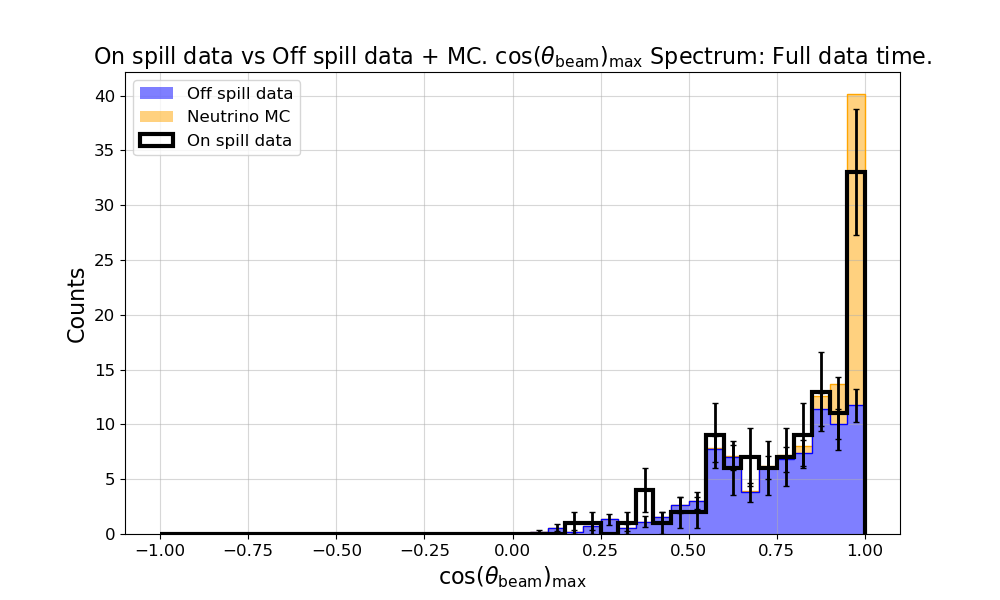
\includegraphics[width=0.49\linewidth]{sections/plots/version_2/beam_on_vs_off_low_tps/output_test_full_time/sig_bkg_mc_max_directionZ_directionZ2_spectrum_full_sig_time.png}
    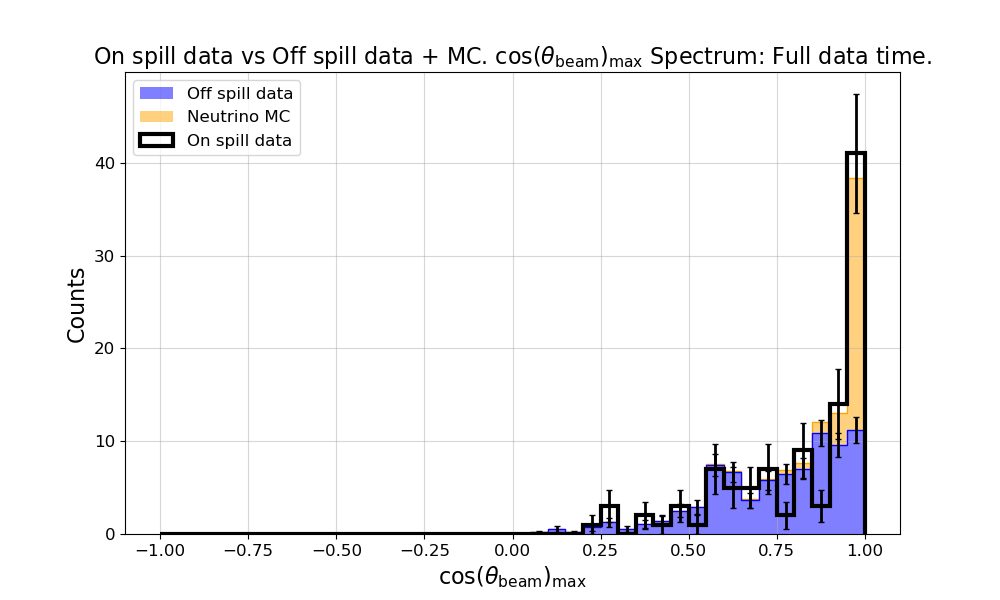
\includegraphics[width=0.49\linewidth]{sections/plots/version_2/beam_on_vs_off_high_tps/output_test_full_time/sig_bkg_mc_max_directionZ_directionZ2_spectrum_full_sig_time.png}\\
    
    \caption{Distribution of $\cos(\theta_{\mathrm{beam}})_\text{max}$ with the low TP rate (left) and the high TP rate (right). 
    The final bin contains the same number of events in both cases because the binning in the plot is wider than the real cut applied, hiding the tiny difference. 
    }
    \label{fig:max_cos_theta_high_low}
\end{figure}

After applying all the selection cuts, the rates of events per hour in both beam-on periods are compatible within the uncertainties, showing that the selection is capable of removing the additional contribution. 

\begin{figure}[h]
    \centering
    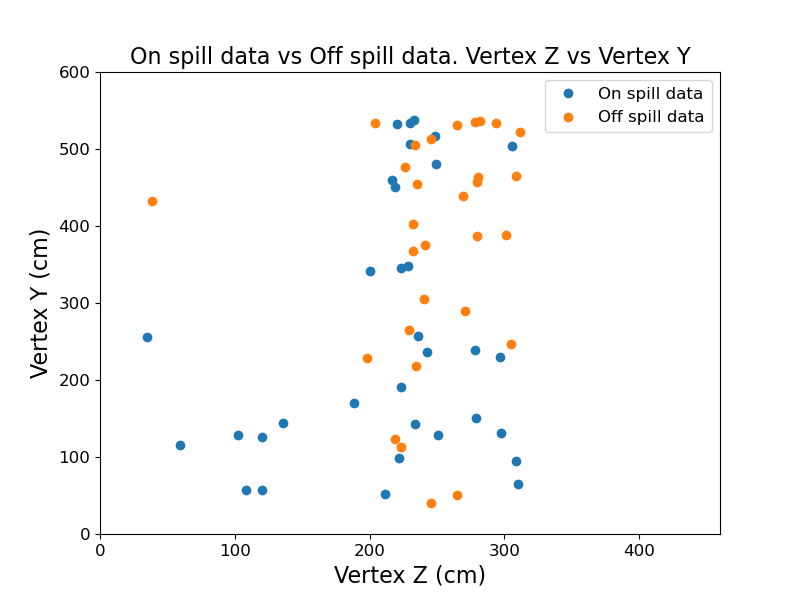
\includegraphics[width=0.69\linewidth]{sections/plots/version_2/beam_on_vs_off_high_tps/sig_bkg_vertexZ_vs_vertexY_scatter.png}
    \caption{Vertex position in the ZY plane for the spill-on and spill-off events that pass all selections, considering the time period with a visible increase in the TP rate corresponding to the beam spill.}
    \label{fig:vertex_position_yz_high_tps}
\end{figure}
\begin{figure}[h]
    \centering
    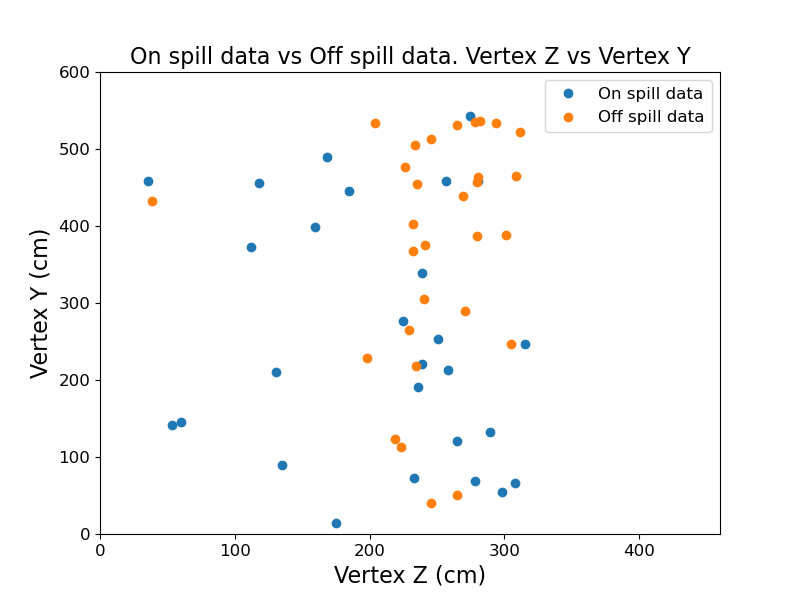
\includegraphics[width=0.69\linewidth]{sections/plots/version_2/beam_on_vs_off_low_tps/sig_bkg_vertexZ_vs_vertexY_scatter.png}
    \caption{Vertex position in the ZY plane for the spill-on and spill-off events that pass all selections, considering the time period without a visible increase in the TP rate (low TP rate).}
    \label{fig:vertex_position_yz}
\end{figure}

As a comparison, the vertex positions in the ZY plane are plotted, and even in this case it is possible to see that the vertices are evenly distributed in the volume along Z and in the lower part of the detector (Figure \ref{fig:vertex_position_yz_high_tps} and \ref{fig:vertex_position_yz}).

The distributions for the other variables of interest are shown, to highlight the fact that the events behave similarly between the time with the high TP rate (Figure \ref{fig:high_tps_beam_on_tail_density}
\ref{fig:high_tps_beam_on_energyDepositedInFifteenth10cm}
\ref{fig:high_tps_beam_on_distance_vertexZ_to_ROI_start}
\ref{fig:high_tps_beam_on_numberOfPFParticles}
\ref{fig:high_tps_beam_on_vertexY}
\ref{fig:high_tps_beam_on_vertexZ}
\ref{fig:high_tps_beam_on_energyDepositedInFifth10cm}
\ref{fig:high_tps_beam_on_ROI_Z_size}
\ref{fig:high_tps_beam_on_energyDepositedInFirst10cm}
) and the low TP rate (Figure \ref{fig:beam_on_tail_density}
\ref{fig:beam_on_energyDepositedInFifteenth10cm}
\ref{fig:beam_on_distance_vertexZ_to_ROI_start}
\ref{fig:beam_on_numberOfPFParticles}
\ref{fig:beam_on_vertexY}
\ref{fig:beam_on_vertexZ}
\ref{fig:beam_on_energyDepositedInFifth10cm}
\ref{fig:beam_on_ROI_Z_size}
\ref{fig:beam_on_energyDepositedInFirst10cm}).


\begin{table}[htbp]
    \centering
    \begin{tabular}{|c|c|c|c|}
        \hline
         & Number of events & Time (hours) & Hourly rate\\
        \hline
        Beam-on & 27 & 8.464 & 3.19 \\
        \hline
        Beam-off & 30 & 44.6886 & 0.67\\
        \hline
    \end{tabular}
    \caption{Observed number of events that pass all selection cuts, considering the full beam off data and only the beam on time with a low TP rate.}
    \label{tab:post_cut_numbers_low_tps}
\end{table}

Finally, it can be interesting to compute the significance of the excess only considering the low TP rate period, where the number of events that pass all selection cuts is 27 ($\text{N}_{\text{ON}}$) within the 8.464 hours ($\text{T}_{\text{ON}}$) of beam on, as reported in Table~\ref{tab:post_cut_numbers_low_tps}.

\begin{figure}[h]
    \centering
    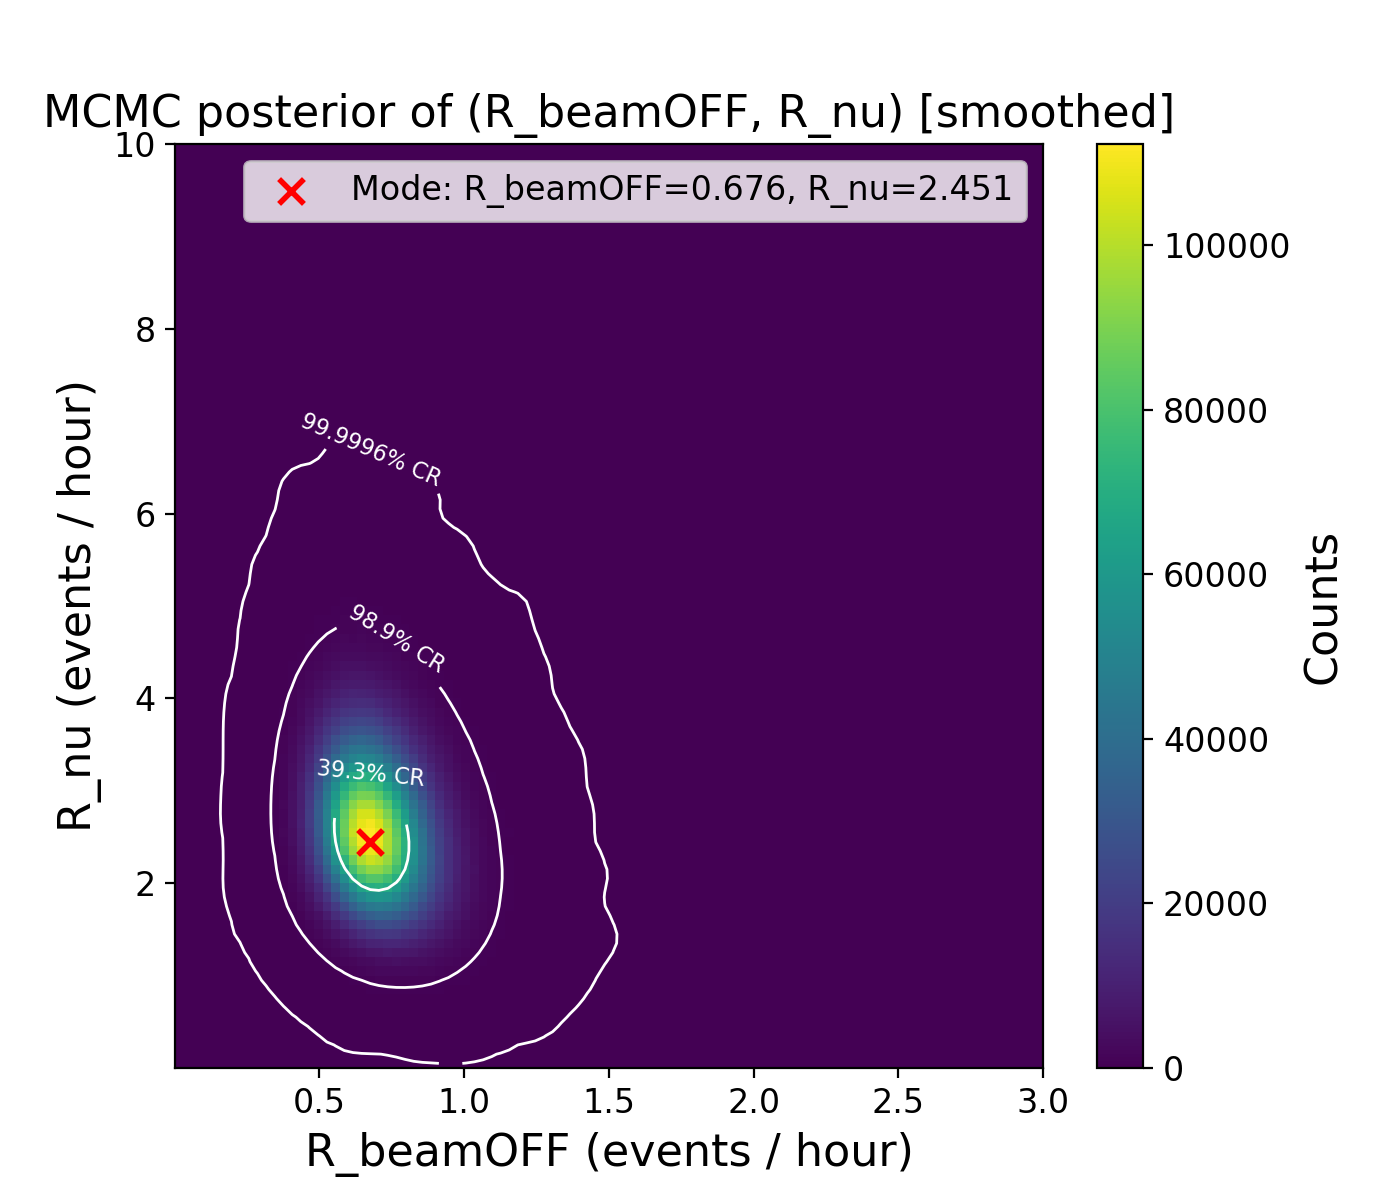
\includegraphics[width=0.69\linewidth]{sections/results/plots/significance/mcmc_posterior_contours_smoothed_low.png}
    \caption{Histogram of the sampled \(\log(\mathcal{L}_{\text{Poisson}})\) using the Monte Carlo method. Contours are drawn using the 0.393, 0.989, and 0.999996 quantiles.}
    \label{fig:mcmc_approach}
\end{figure}

Applying the same statistical method explained in Section \ref{chap:significance_method}, the significance of the excess is computed using Eq.~\ref{eq:basic_formula}, obtaining $6.44\sigma$.
Then, again following the strategy explained previously, the likelihood is sampled using a MCMC method and the contours are drawn using the 0.393, 0.989, and 0.999996 quantiles. Even with the reduced statistics, the hypothesis \(\text{R}_{\text{neutrino}}=0\) falls outside of the credible region at 99.9996\% probability, for every plausible true \(\text{R}_{\text{background}}\).


\clearpage
